\chapter{Datasets}

We perform several experiments and ablation studies on some gaze tracking datasets in order to demonstrate the versatility of our method. There are three datasets used in this work which vary in terms of their nature (regression versus classification), ground truths (2-Way versus 3-Way), and the curation methodologies adopted (well-curated versus uncurated), which are discussed in the next sections.


%%%%%%%%%%
\section{3-Way UK Dataset}
This dataset is collected in the UK from an \href{https://drive.google.com/file/d/124HQbKAsR6YVIeK-IArFKTnjU8MRNNjh/view?usp=sharing}{Android app developed by Aditya Modi} from our team for the creation of the 3-Way gaze classification dataset. The app displays some objects in the left, middle and right regions of the screen, one at a time, as shown in figure \ref{fig:3wayUKdata}. The subject is asked to keep tracking the object as it appears on the screen in different regions while the front camera records the face of the subject.

\begin{figure}[h]
  \centering
    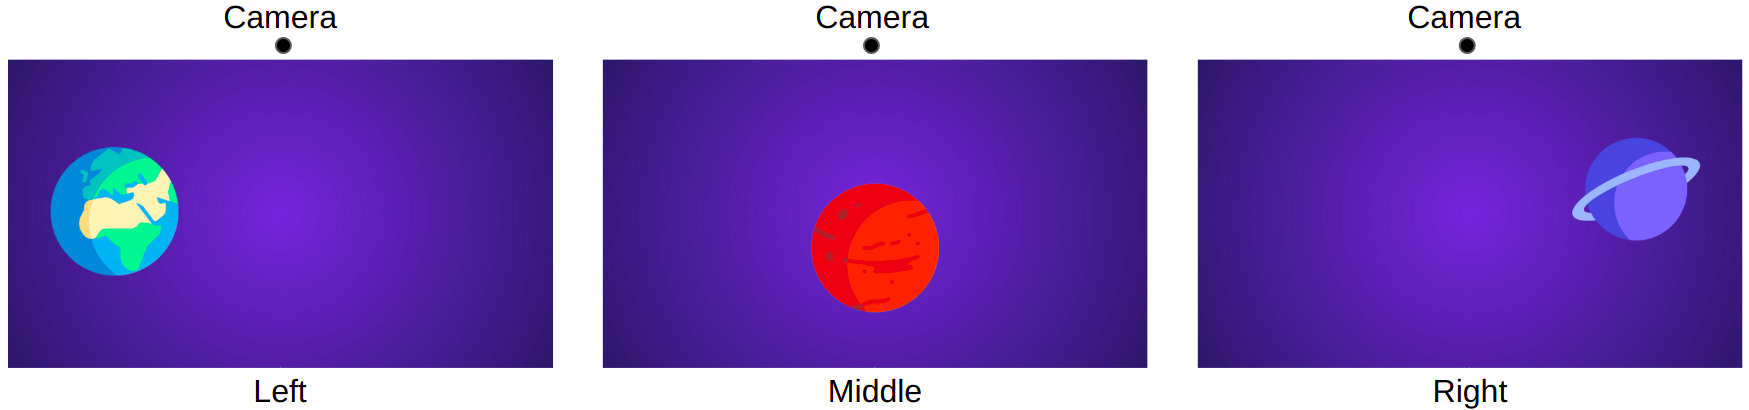
\includegraphics[width=0.8\textwidth]{Dataset/3-Way_UK_dataset}
    \caption{3-Way UK Dataset}
    \label{fig:3wayUKdata}
\end{figure}

\begin{figure}[h]
  \centering
    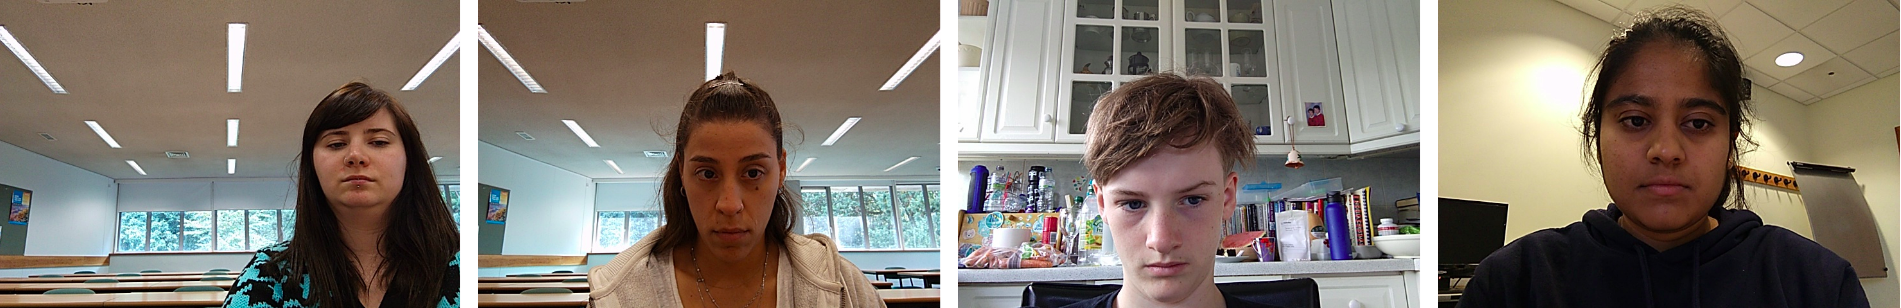
\includegraphics[width=1.0\textwidth]{Dataset/3Way_UK_subjects}
    \caption{Some examples from 3-Way UK Dataset}
    \label{fig:3wayUKdata_examples}
\end{figure}

It contains one of the three-class labels (Left, Middle, or Right) for each image frame. The device used for the collection of data is Huawei MediaPad M3 Lite 10 tablet (also referred to as \emph{UK device} here onwards). The camera in this device is located at the center of the long edge of the screen. The camera location is an important factor in the device specifications because the gaze of the subject (either XY coordinates or gaze classes) are defined w.r.t. the camera. In case of XY coordinate regression, the origin is defined at the camera location, and in the case of gaze classification, the divisions of the screen region are assigned taking into consideration the location of the camera.

The dataset contains 23 different subjects (samples shown in figure \ref{fig:3wayUKdata_examples}), each performing the task several times at different locations and in different lighting conditions, poses, etc. It contains a total of 539508 frames which are split into the train, val and test in a ratio of approximately 7:1:2 with 369835, 51998, and 117675 frames, respectively.


%%%%%%%%%%
\section{Filtered 2-Way UK Dataset}
Since we are also interested in 2-way along with 3-way gaze classification, we prepare a customized version of the 2-way gaze classification dataset from the 3-way UK dataset by simply removing the frames with "Middle" as the ground truth. Note that the resulting 2-way dataset has a buffer region in the middle where there are no frames in the dataset. So in that sense, it is a well-curated dataset.

The resulting dataset contains a total of 420811 frames which are split into the train, val and test in a ratio of approximately 7:1:2 with 288477, 40555, and 91779 frames, respectively.


%%%%%%%%%%
\section{2-Way Nottingham START Dataset}
The 2-way Nottingham START dataset is created by the Preferential Looking task being performed by children as a part of the START project in Nottingham. The app displays a social and a non-social video clip simultaneously on the screen; one displayed on the left and the other on the right side of the screen, randomly, as shown in figure \ref{fig:2waySTARTdata}. By recording the face and gazes of the children, this task gauges the social preference of the children.

% \begin{figure}[h]
%   \centering
%     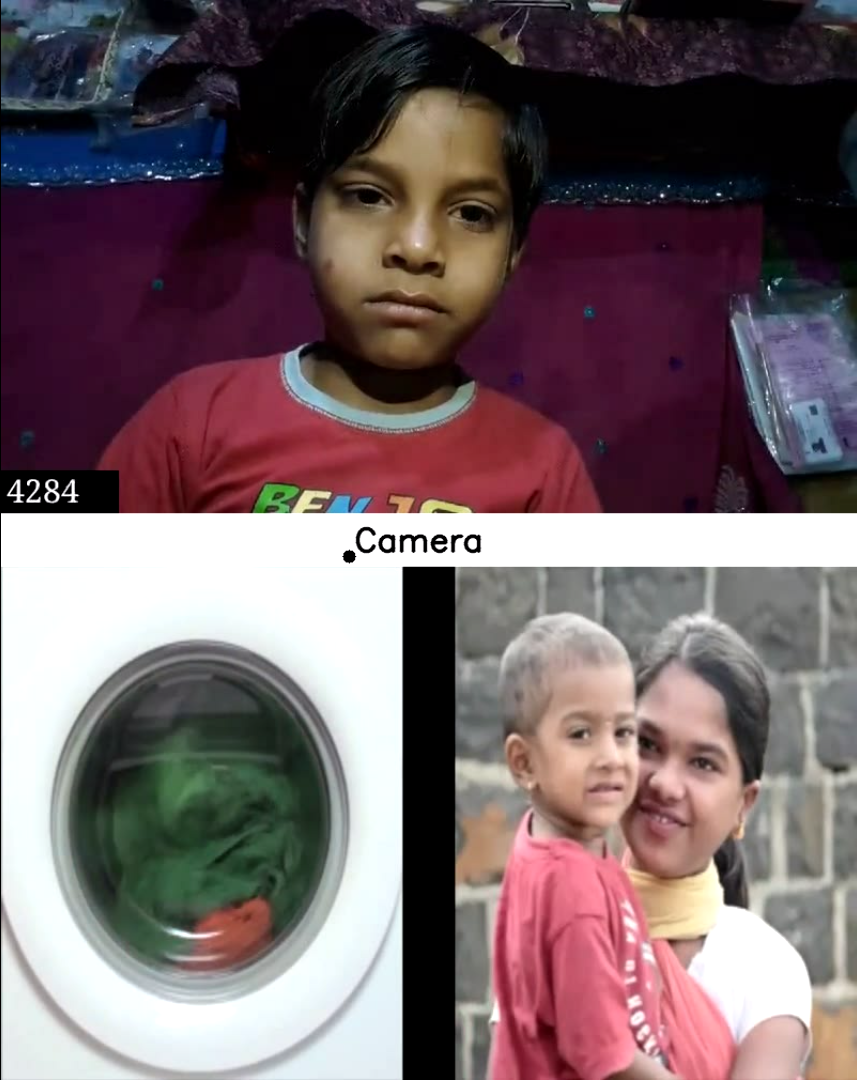
\includegraphics[width=0.38\textwidth]{Dataset/2-Way_START_dataset}
%     \caption{2-Way START Dataset}
%     \label{fig:2waySTARTdata}
% \end{figure}

\begin{figure}[h]
    \centering
    \captionsetup[subfigure]{justification=centering}
    \subfloat[Preferential Looking task]{{
        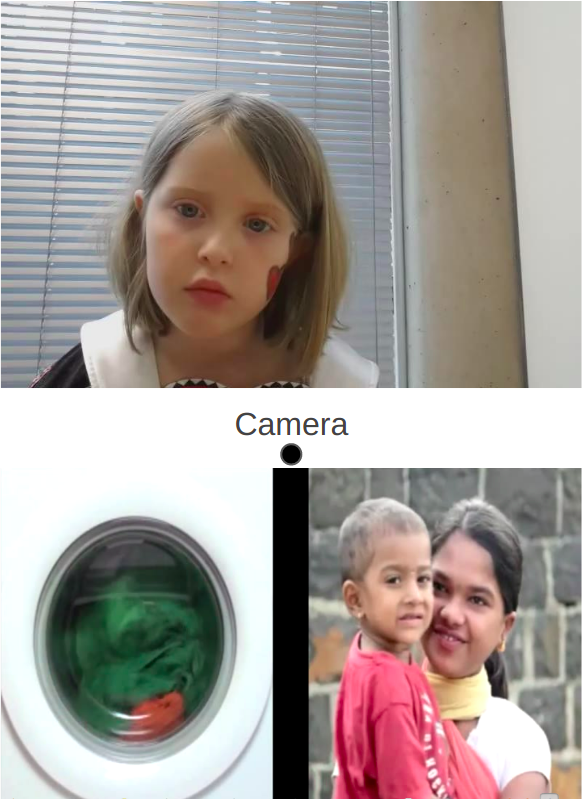
\includegraphics[width=0.3\textwidth,valign=m]{Dataset/2Way_Nottingham_START}
        }}
    \quad
    \subfloat[3rd person view of Preferential Looking task]{{
        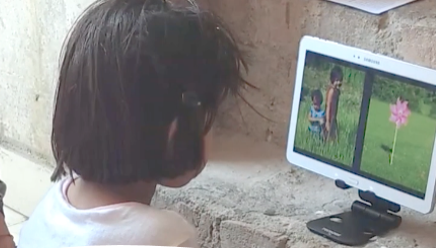
\includegraphics[scale=0.25,valign=m]{Dataset/3rdPersonView_PrefLooking}
    }}
    \caption{2-Way START Dataset collected using Preferential looking task}
    \label{fig:2waySTARTdata}
\end{figure}

It contains one of the two class labels (Left or Right) for each image frame. The device used for the collection of data is Samsung Note 10 SM P600 tablet (also referred to as \emph{START device} here onwards). The device dimensions are 24 cm x 17 cm and the camera in this device is located at an offset of 2 cm towards the left from the center of the long edge of the screen. Note that this dataset is not an in-the-wild dataset purely because although the START app was used for dataset collection, the videos were recorded in a lab environment.

The dataset contains 11 different subjects, each performing the Preferential Looking task. It contains a total of 7917 frames which are split into the train, val and test in a ratio of approximately 7:1:2 with 5541, 791, and 1585 frames, respectively.